%-----------------------------------------------------
%----- Setup -----------------------------------------
%-----------------------------------------------------
% for normal version
\documentclass[xcolor=dvipsnames]{beamer}
% for trans version
%\documentclass[xcolor=dvipsnames, trans]{beamer}
%\usepackage{pgfpages}
%\pgfpagesuselayout{2 on 1}[a4paper,border shrink=10mm]

%-----------------------------------------------------
%----- Document begins
%-----------------------------------------------------
\usetheme{Warsaw}
\setbeamertemplate{navigation symbols}{}

\usepackage[T1]{fontenc}
%\usepackage[utf-8]{inputenc}
\usepackage{lmodern}
\usepackage[english]{babel}

\usepackage{mathpazo}
\usepackage{graphicx}
\usepackage[labelformat=empty, labelsep=none,
  font=footnotesize]{caption}
\usepackage{sidecap}
\usecolortheme[named=Bittersweet]{structure}
\usepackage{array}
\usepackage{multirow}
\usepackage{amsmath}
\usepackage{stmaryrd}
\usepackage{graphicx}
\usepackage{bm}
\setbeamercovered{transparent}

% Shorthand for bold math
\def\B#1{\bm{#1}}
% Matrix transpose
\def\trans{^\mathsf{T}}
% A compact fraction
\def\slantfrac#1#2{\kern.1em^{#1}\kern-.1em/\kern-.1em_{#2}}
% "off" indice
\def\off{\text{off}}
% cholesky decomposition
\def\chol{\text{chol}}

\title[NeuroBreakfast - \today\hspace{\stretch{1}}
  (\insertframenumber{}/\inserttotalframenumber{})]{Solving two-person zero-sum sequential games
via efficient computation of Nash equilibria: proof-of-concept on Kuhn's 3-card Poker}
\author{DOHMATOB Elvis \inst{1,2}}
\institute{
  \inst{1}Parietal Team, INRIA\\\inst{2}Universit\'e Paris-Sud}

\date{} \selectlanguage{english}
\begin{document}

\begin{frame}
\maketitle
\end{frame}

%\logo{\includegraphics[scale=0.1]{img/logo_parietal.png}}
\begin{frame}
  \frametitle{Problem}
  Given a \textcolor{orange}{sequential two-person zero-sum game} (e.g Texas Hold'em Poker), construct an \textcolor{orange}{optimal player}.
  %% Approximate the population covariance matrix $\Sigma$ from $n$ samples.
  %% \begin{itemize}
  %% \item $\B{S}$ is the $p \times p$ sample covariance
  %%   matrix.\\
  %%   $\B{S} = \frac{1}{n}\sum^n_{i=1}x_ix_i\trans$. $\mathbb{E}[S] = \Sigma$.
  %% \item Largest (resp. smallest) eigenvalue of $S$ is biased upwards
  %%   (resp. downwards)
  %% \item $\Rightarrow$ Shrinkage: pushing up (resp. pulling down) the
  %%   largest (resp. smallest) eigenvalue. \textcolor{gray}{(Stein
  %%     1976)}.
  %% \end{itemize}

  %% \vfill

  %% Ledoit-Wolf problem:\\
  %% \begin{itemize}
  %% \item $\underset{\hat{\B{\Sigma}}}{\min} \,
  %%   \mathbb{E}\left\{\|\hat{\B{\Sigma}}(\{x_i\}^n_{i=1}) - \B{\Sigma}\|^2_F\right\}$ with $\|\B{A}\|_F = \sqrt{\text{Tr}(\B{A}\B{A}\trans)/p}$
  %% \end{itemize}
\end{frame}

\begin{frame}
  \frametitle{Two-person zero sum Sequential games}
  \uncover<1->{
  \begin{itemize}[<+->]
      \item There are 3 players: \textcolor{blue}{nature (player 0)}, \textcolor{red}{Alice (player 1)}, and \textcolor{green}{Bob (player 2)}.}
    \item Players take turns in making moves
    \item Sets of moves of any two distinct players don't
      overlap (i.e \textcolor{red}{$A_p \cap A_q = \emptyset$ if $p \ne q$})
  \end{itemize}
\end{frame}

\begin{frame}
\frametitle{Strategy profiles, simplexes and complexes}
\begin{definition}
  \begin{itemize}[<+->]
    \item The \textcolor{blue}{$n$-\textit{simplex}}, denoted $\Delta_n$, is the subset of $\mathbb{R}^{n+1}$ defined by
      \begin{equation}
        \Delta_n := \left\{x \in \mathbb{R}^{n+1}\text{ }|\text{ } x_i \ge 0\text{ } \forall i, \text{ and } \sum_{i=1}^{n+1}{x_i} = 1\right\}
      \end{equation}
    \item Each kink $\delta_i := (0, ..., 0,1,0, ...,0)$ of $\Delta_n$ represents a \textit{\textcolor{blue}{pure-strategy}}.
      Any non-kink point $x$ of $\Delta_n$ represents a
      \textit{\textcolor{blue}{mixed-strategy}}. Thus $\Delta_n$ is simply the \textit{convex hall} of $(n+1)$-dimensional pure strategies $\delta_i$.
    \item A \textit{\textcolor{blue}{complex}} is an abstract \textit{\textcolor{blue}{polyhedron}} whose kinks are themselves simplexes. Points on
      a complex correspond to \textit{\textcolor{blue}{behavioural strategies}}.
  \end{itemize}
\end{definition}
\end{frame}

\begin{frame}
\frametitle{Simplexes and complexes (examples of)}
%% \begin{figure}
%%   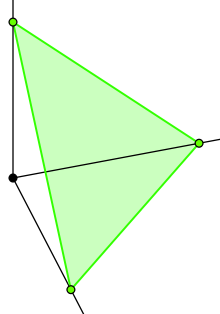
\includegraphics[width=3cm]{simplex.png}
%%   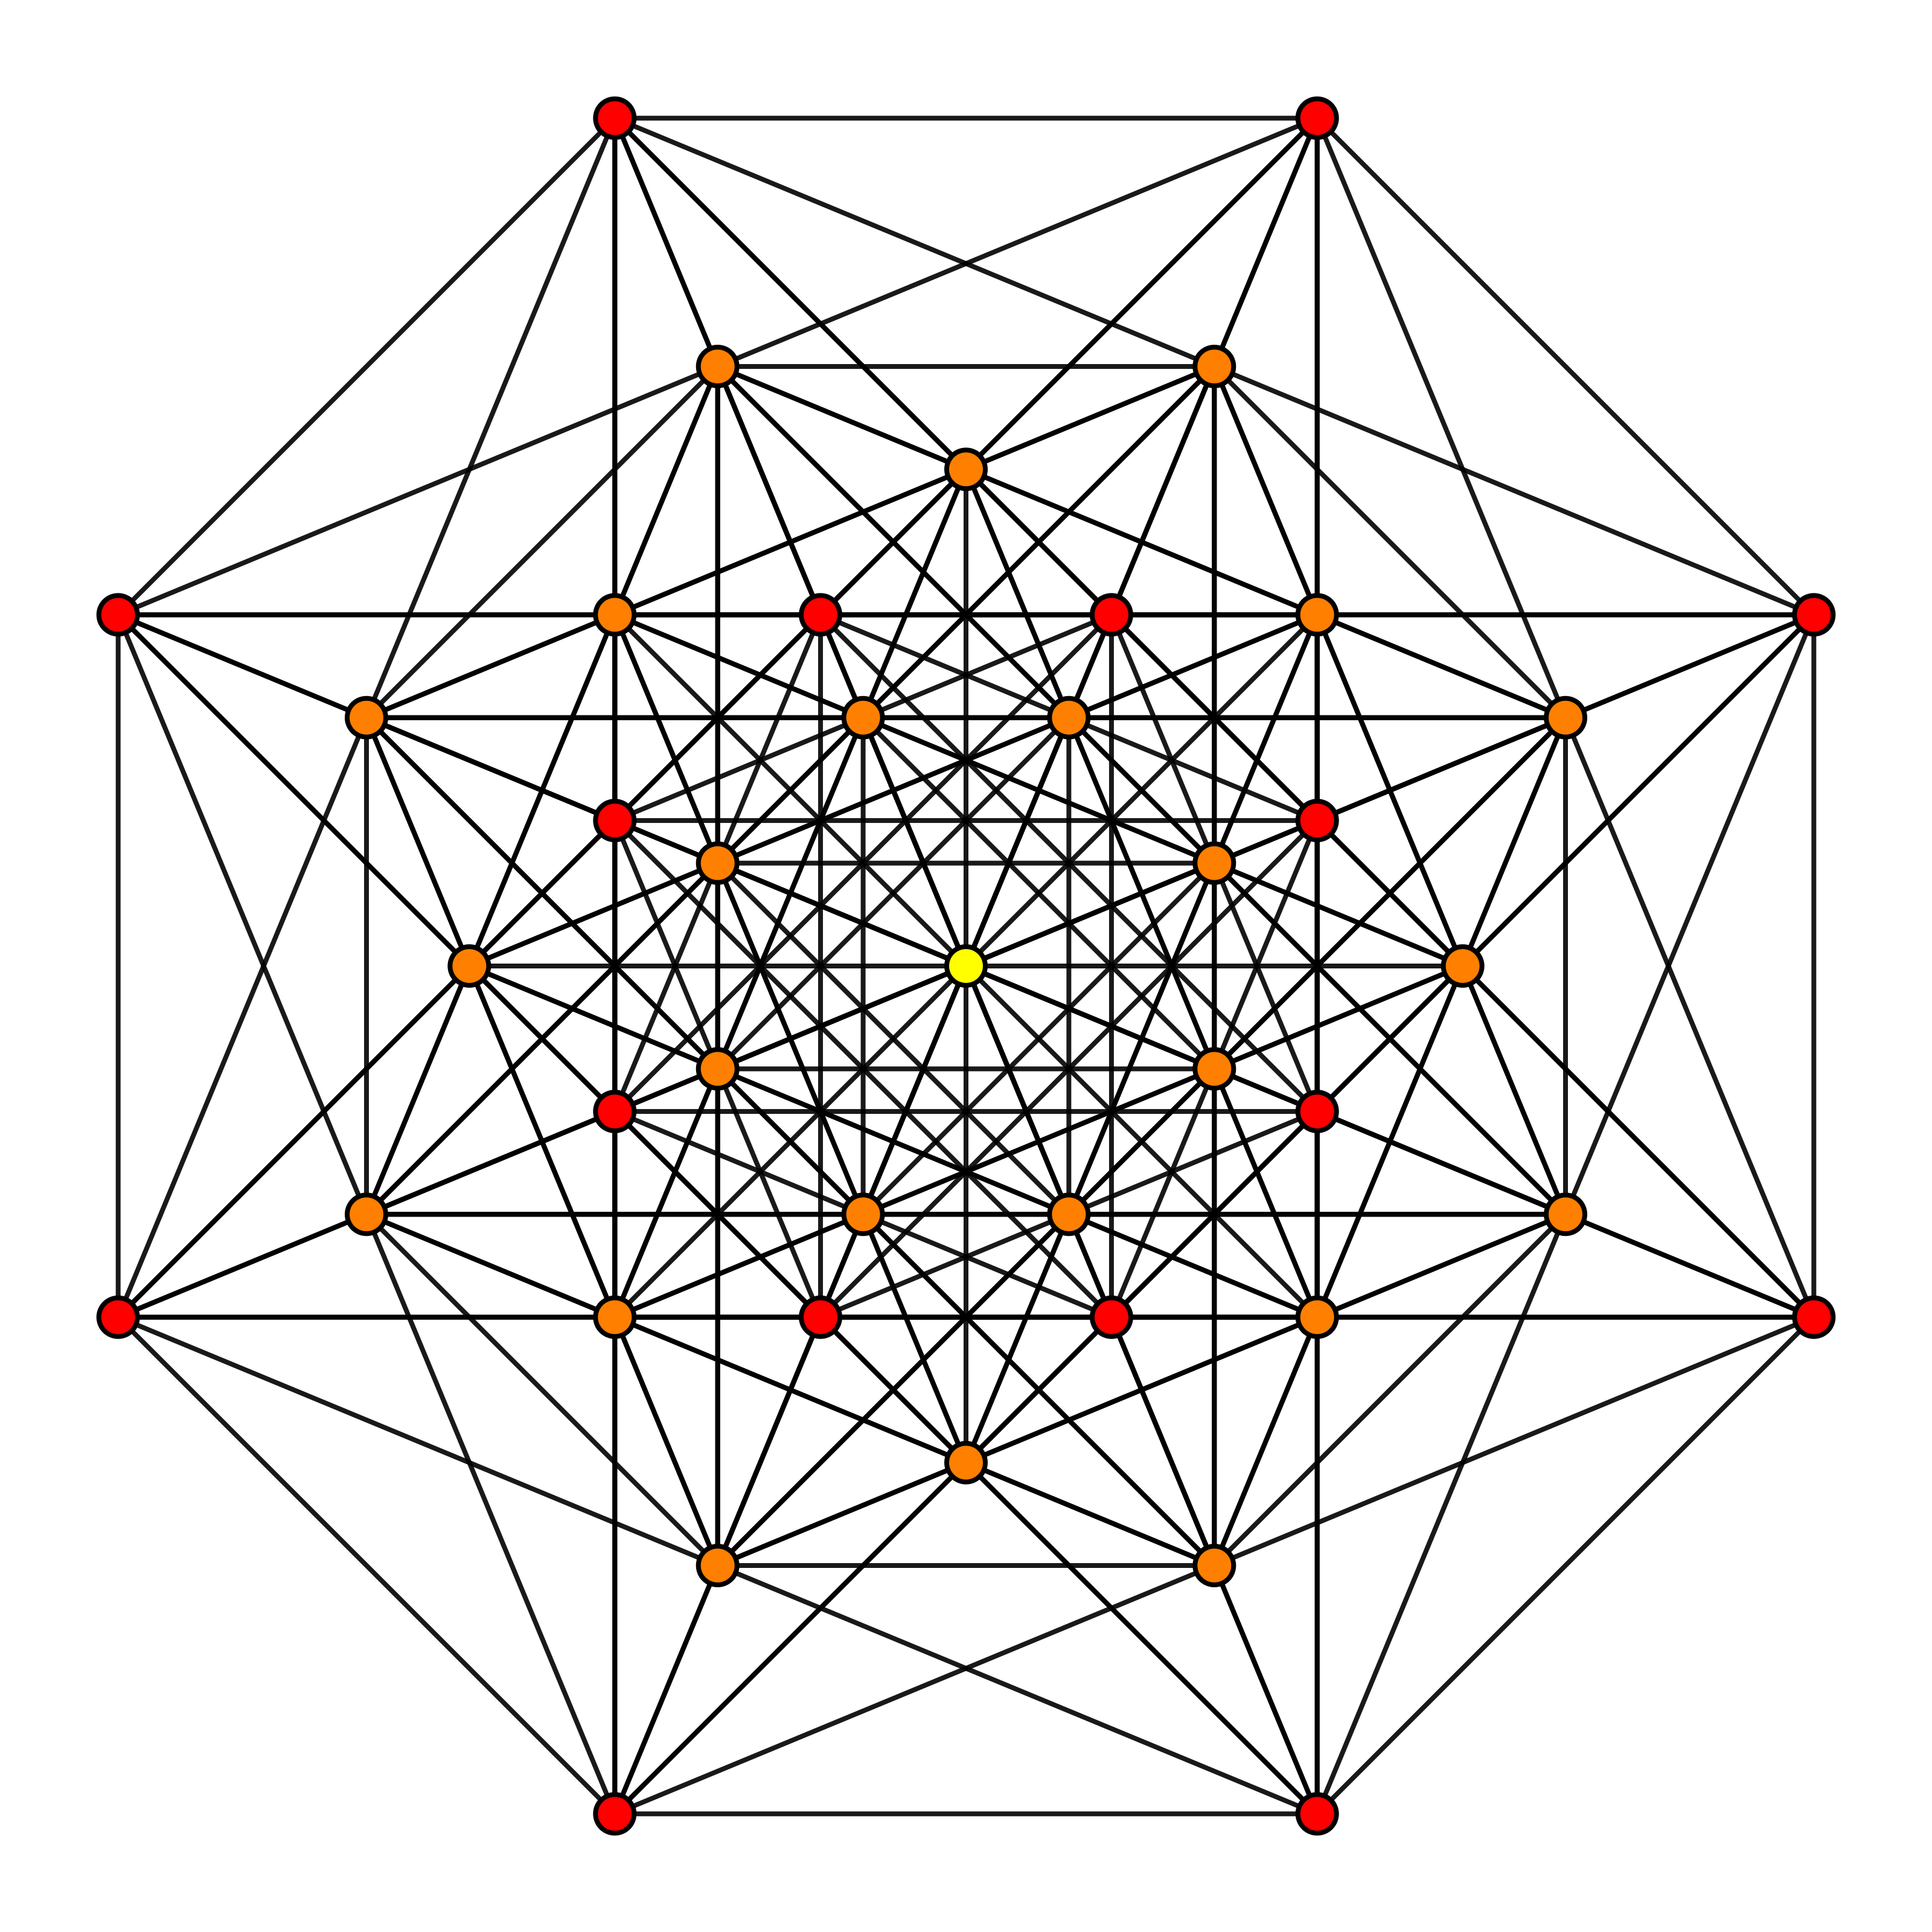
\includegraphics[width=3cm]{7-simplex.png}
%%   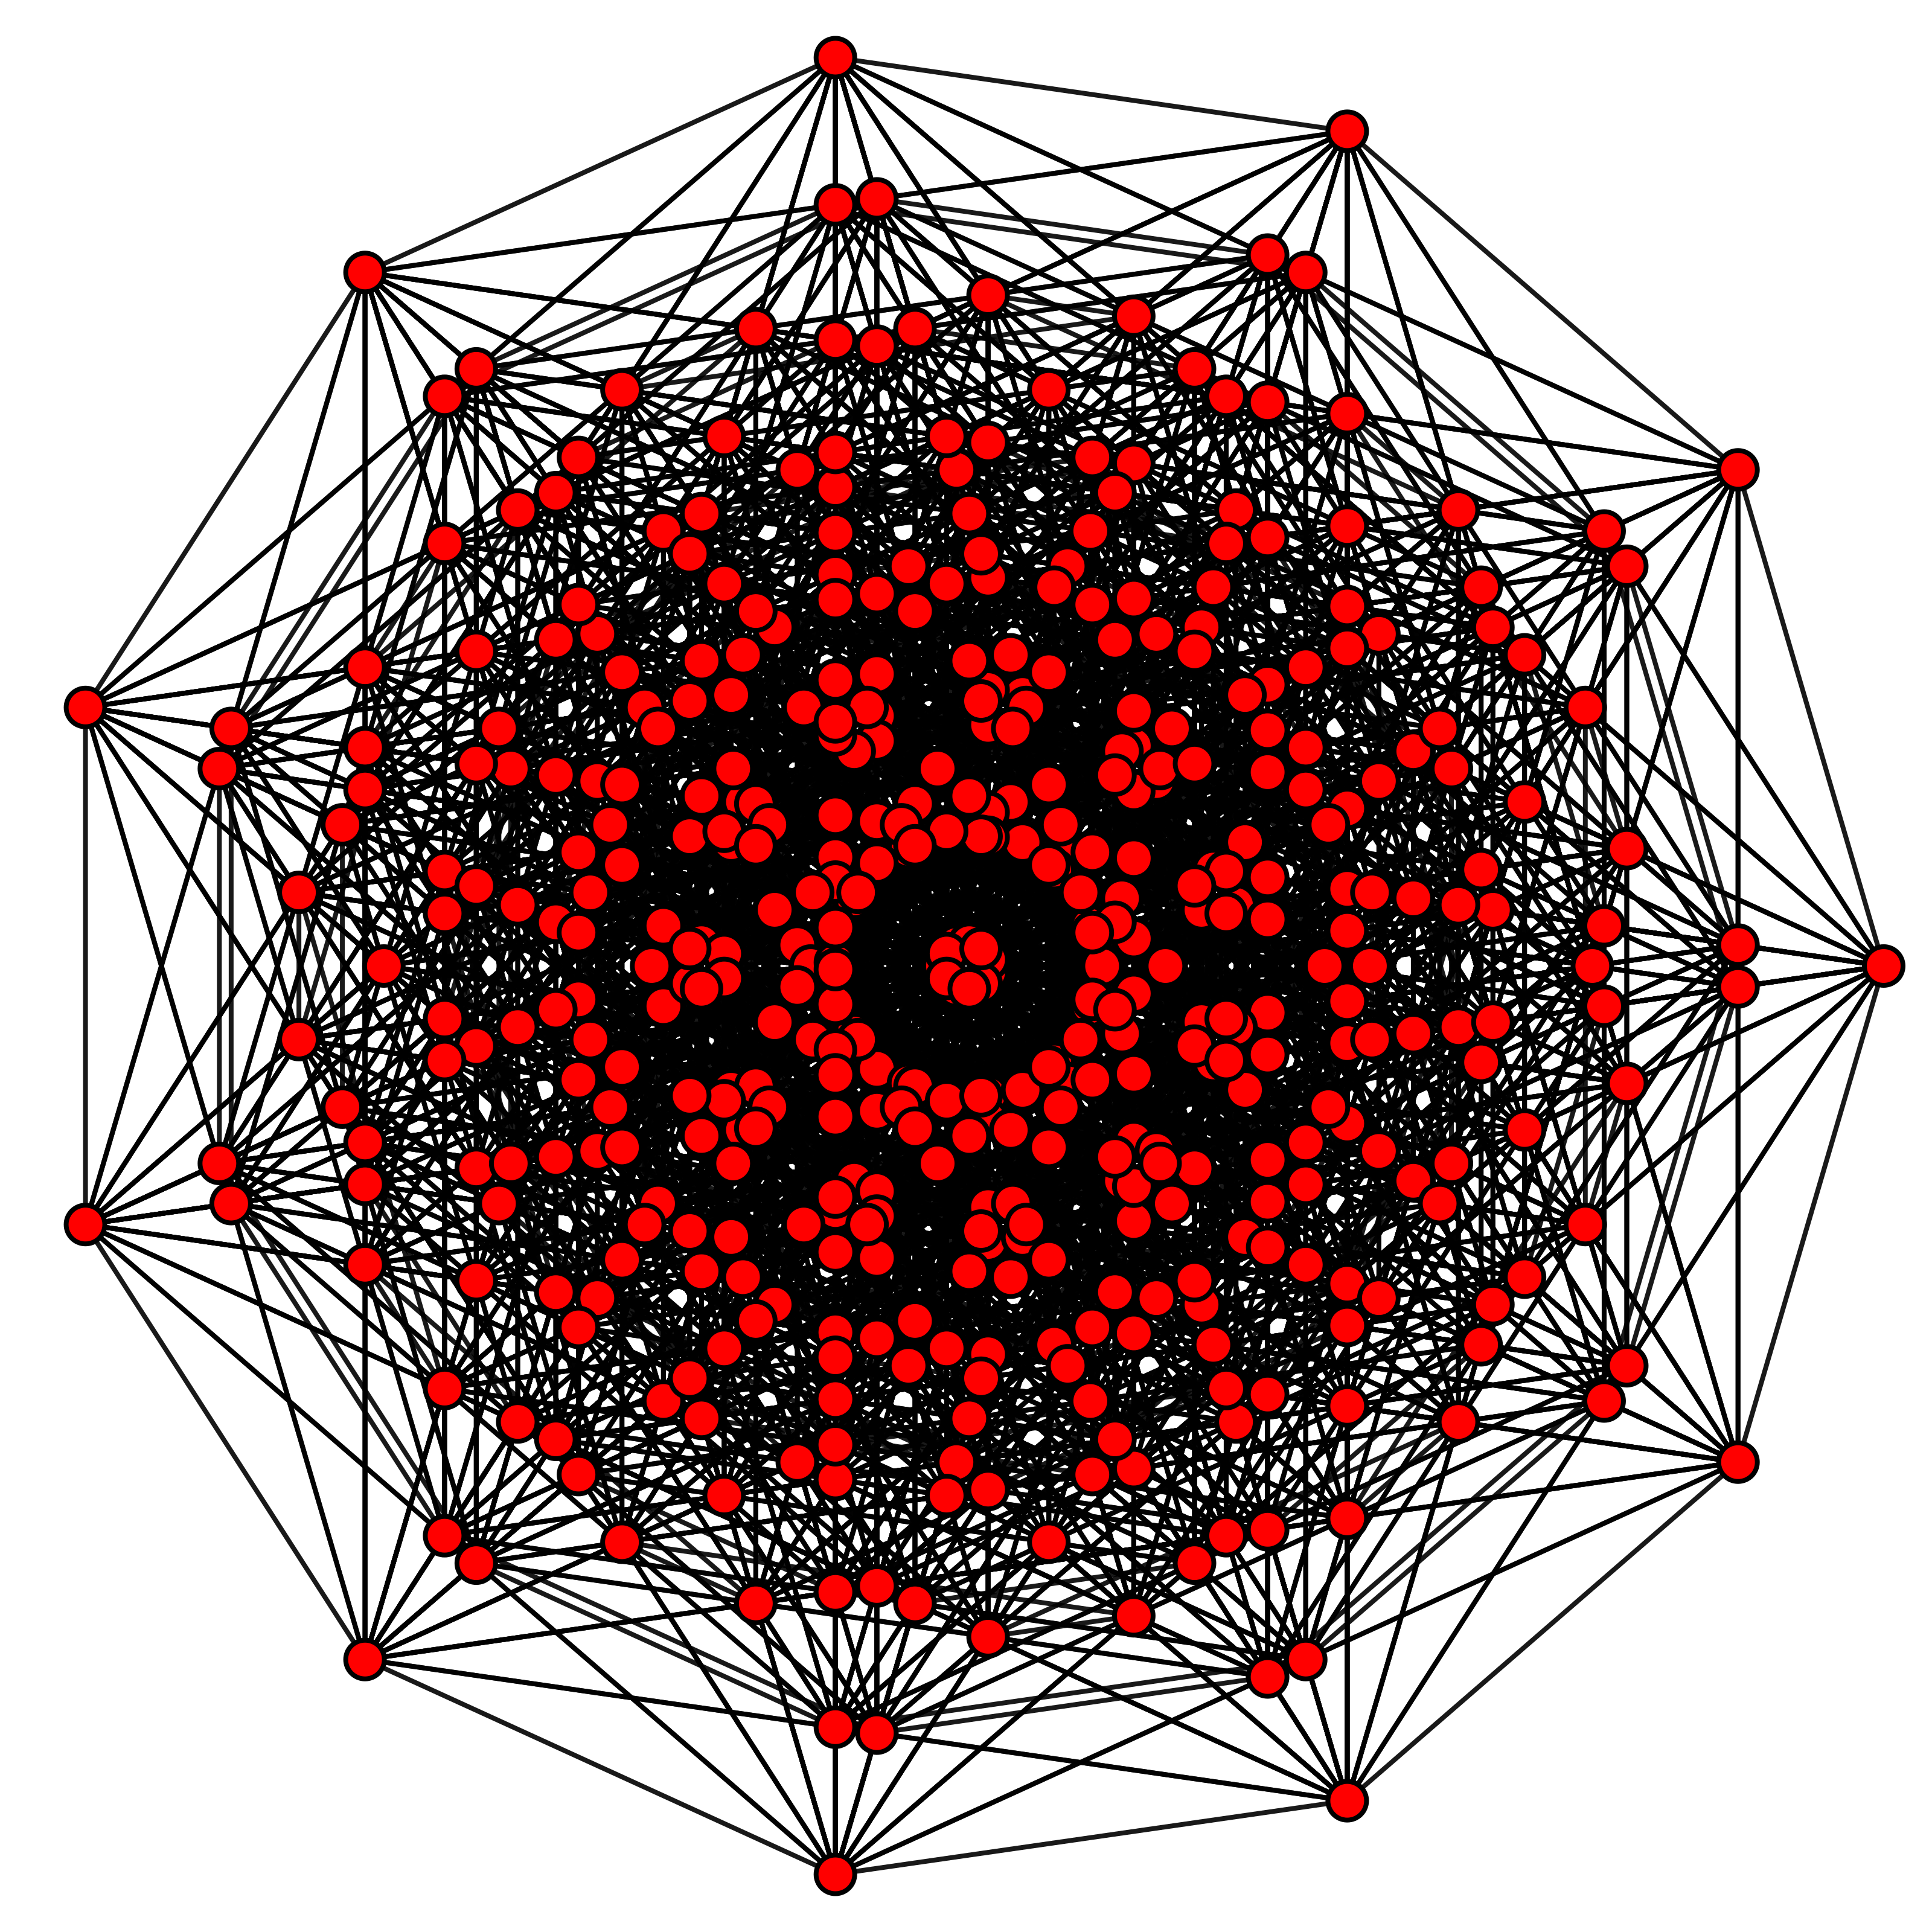
\includegraphics[width=3cm]{10-simplex.png}
%%   \caption{\textbf{Left}: 2-simplex \textbf{Middle}: 7-simplex \textbf{Right}: 10-simplex}
%% \end{figure}
\end{frame}

\begin{frame}
  \frametitle{NE minimax and best-response in sequential-games}
Thanks to the sequence-form representation, we have:
\begin{itemize}[<+->]
\item NE problem for Alice and Bob is the the \textit{\textcolor{blue}{saddle-point problem}}
  \begin{equation}
    \underset{x \in Q_1}{maximize}\text{ }\underset{y \in Q_2}{minimize}\text{ }y^TAx,
    \label{eq:minimax_stengel}
  \end{equation}
  
    where:
   \begin{equation}
     \left .
     \begin{split}
       Q_1 &:= \{x \in \mathbb{R}_+^n\text{ }|\text{ }Ex=e\} \text{ is \textcolor{blue}{Alice's complex, and}}\\
       Q_2 &:= \{y \in \mathbb{R}_+^m\text{ }|\text{ }Fy=f\} \text{ is \textcolor{red}{Bob's complex}.}
     \end{split}
      \right\}
   \end{equation}
   A saddle-point $(x^*, y^*)$ corresponds to a NE for the game.
   \item Given a fixed behavioural strategy $y_0 \in Q_2$ for Bob, a \textit{\textcolor{blue}{best-response}} behavioural strategy $x_0$ for Alice
     \footnote{Of course, there is an analogous concept for Bob.}
    is a solution to the LCP
    \begin{equation}
      \underset{x\in Q_1}{maximize}\text{ }{y_0^TAx}
    \end{equation}
  \end{itemize}
\end{frame}
    
    \begin{frame}
  \frametitle{Two-person zero sum Sequential games}
  \begin{itemize}[<+->]
    \item The game tree $T$ (from Alice's perspective) is defined as follows.
    $T$ has a set $V(T)$ of nodes (aka vertices) and a set $E(T)$ of edges.
    \item Each node $v$ belongs to a single player, $p(v)$, called "\textcolor{blue}{the player to act
    at $v$}"; $p(v) := 3$ if $v$ is a leaf node. At node $v$, the player $p(v)$ has a set
    $C(v) \subset A_p$ of possible moves.
    \item For each player $p \in \{0, 1, 2\}$,
      the set of all nodes at which $p$ acts is called the nodes of $p$,
    denoted $V_p(T)$.% Thus $v(0)$, $v(1)$, and $v(2)$ form a partition of $V(T)$.
  \item There are two kinds of nodes: the \textcolor{blue}{leaf nodes} $L(T)$, at which the game must
    end and \textcolor{blue}{decision nodes} $D(T)$, at which the player to act must make a move.
    \textcolor{orange}{For example in Poker,
    a leaf node is reached at countdown, or when a player folds, or when the
    player runs out of money.}
    \item  There is a special node \textcolor{blue}{root}(T) defined by $root(T) := (/, p_0)$,

    \item In accordance with the rules of the game, every other node
      $y \in V(T)-\{root(T)\}$ is of the form $y = v.(c, p(v))$

  \end{itemize}
\end{frame}
  
\begin{frame}
  \frametitle{Sequences and payoff matrix}
  \begin{itemize}[<+->]
    \item Let $S_p$ be the sequences of moves for player $p$. Then any $\sigma \in S_p$ is either the empty sequence $\empty$ set or can be written as $\sigma_{h_p} c$ where $h_p$ is an information set of $p$ and $c$ is a choice at $h_p$.
      \item Precisely,
        \begin{equation}
          S_p = \{\emptyset\} \cup \{\sigma_{h}c\text{ }|\text{ }h \in H_{p}, c \in C_h\}
        \end{equation}
        \item The payoff matrix $A = (a_{\sigma,\tau})$ by
          \begin{equation}
            a_{\sigma,\tau} := \sum_{\text{leaf }t:\text{ } \sigma_1(t) = \sigma, \sigma_2(t) = \tau}\beta_0(\sigma_0(t))a(t)
            \end{equation}
  \end{itemize}
\end{frame}

\begin{frame}
  \frametitle{NE computation Kuhn's Poker}
  \[   E = \left( \begin{array}{ccccccccccccc}
1&0&0&0&0&0&0&0&0&0&0&0&0\\-1&0&0&0&0&0&0&0&0&1&0&0&1\\-1&1&0&0&1&0&0&0&0&0&0&0&0\\-1&0&0&0&0&1&0&0&1&0&0&0&0\\0&-1&1&1&0&0&0&0&0&0&0&0&0\\0&0&0&0&0&-1&1&1&0&0&0&0&0\\0&0&0&0&0&0&0&0&0&-1&1&1&0
\end{array} \right),\]
  $e = (1, 0, 0, 0, 0, 0, 0)$

  %% \begin{figure}
  %%   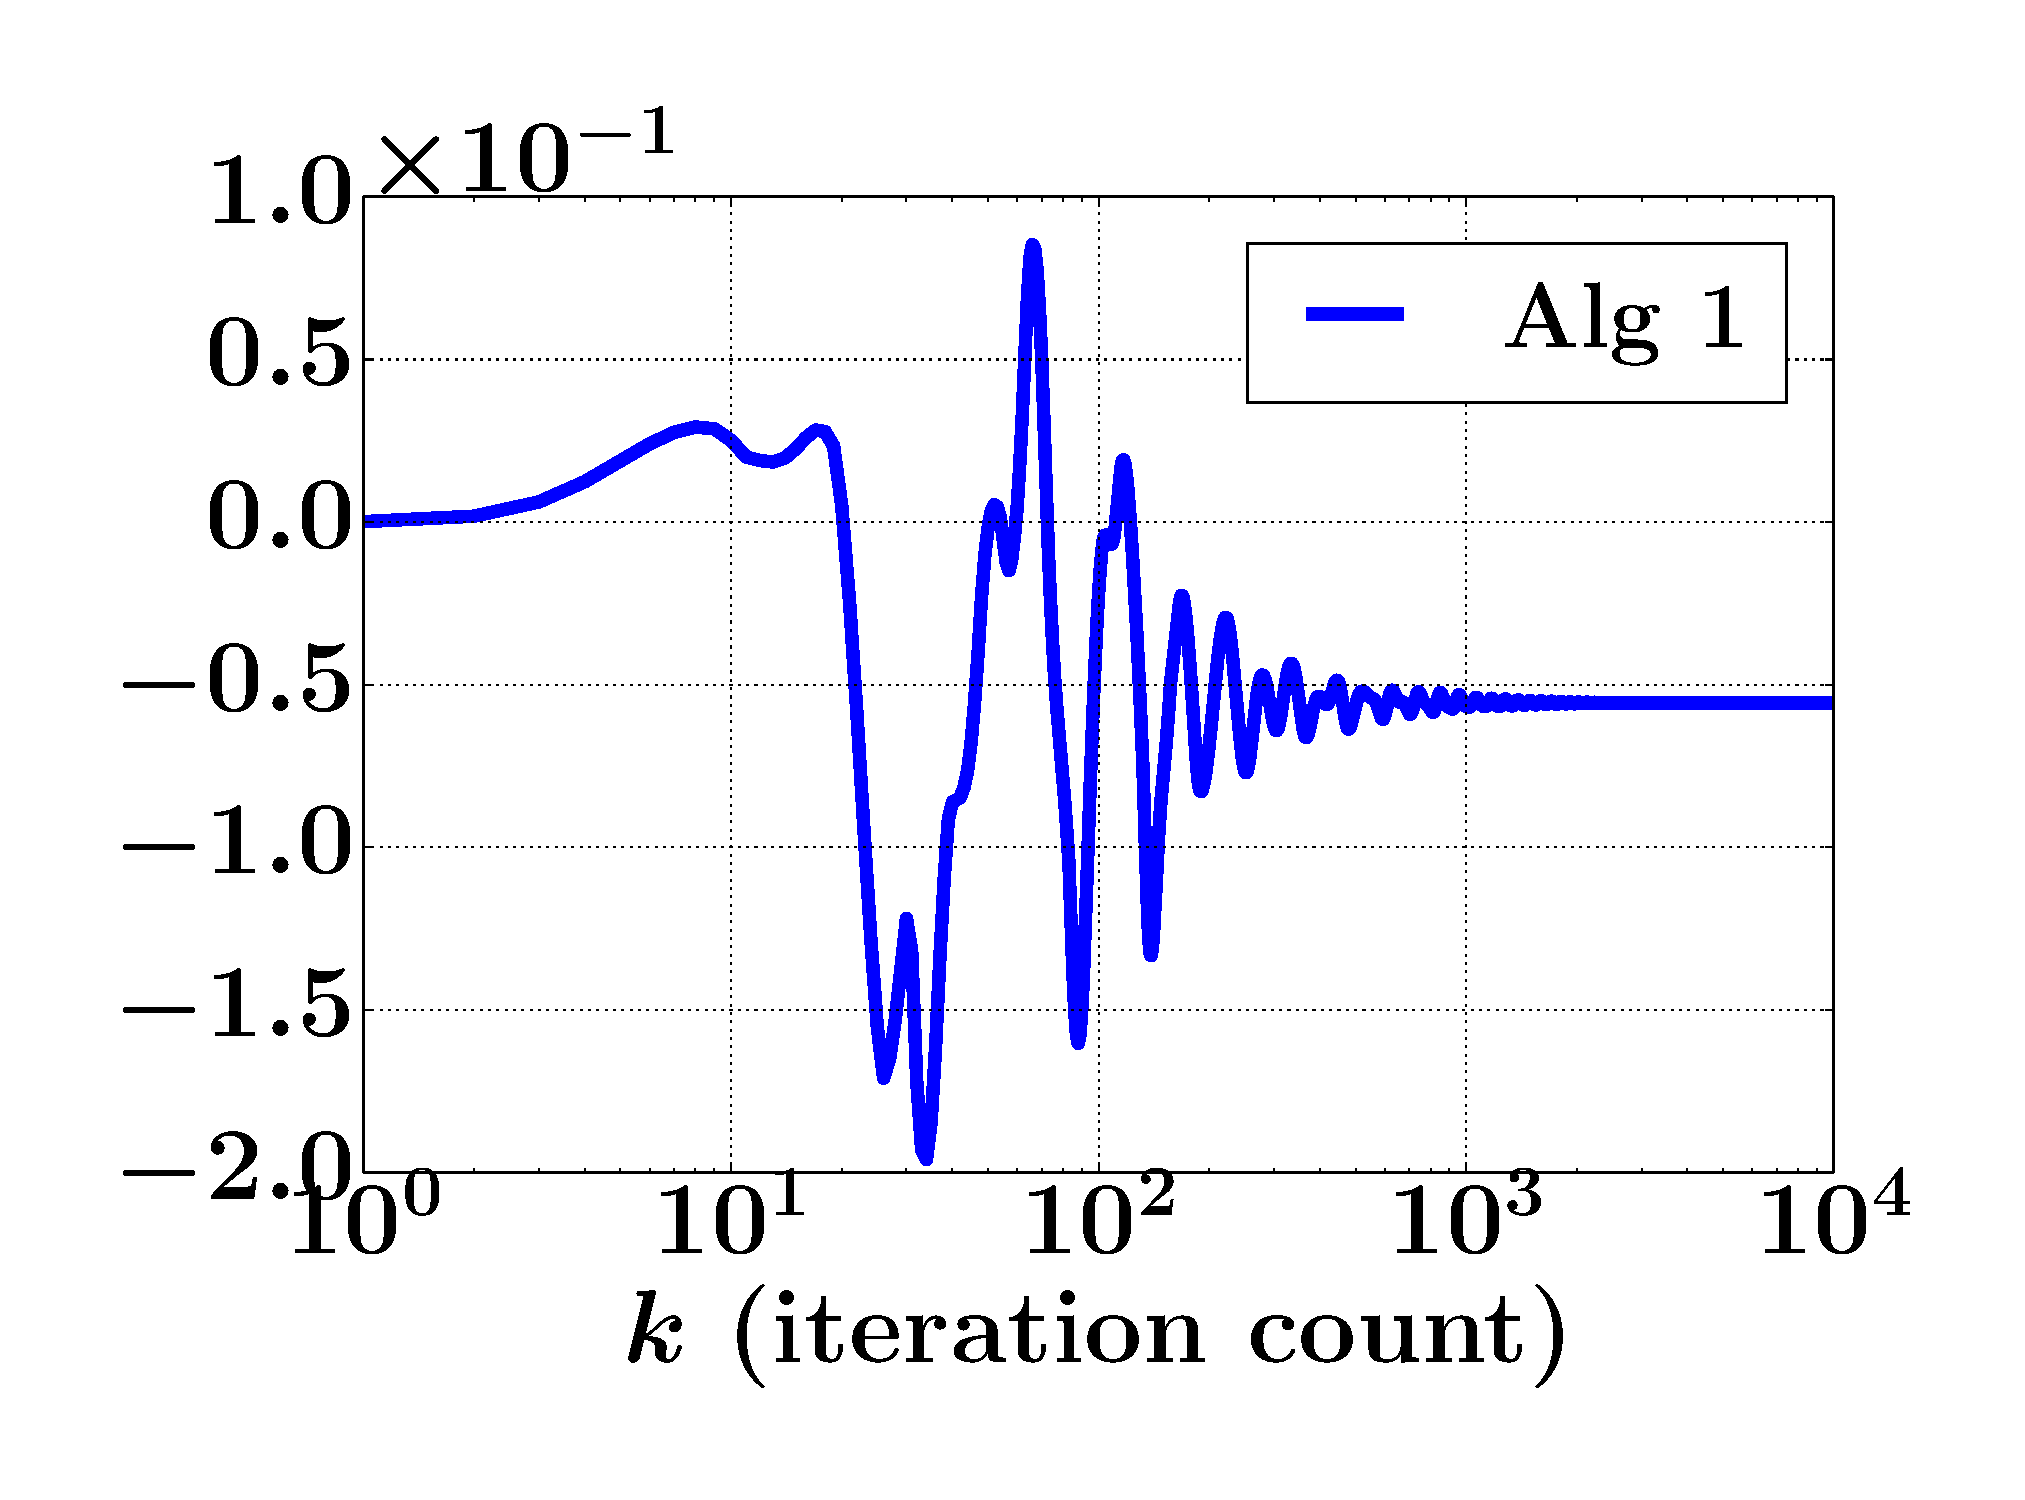
\includegraphics[width=7cm]{Kuhn3112_NE.pdf}
  %%   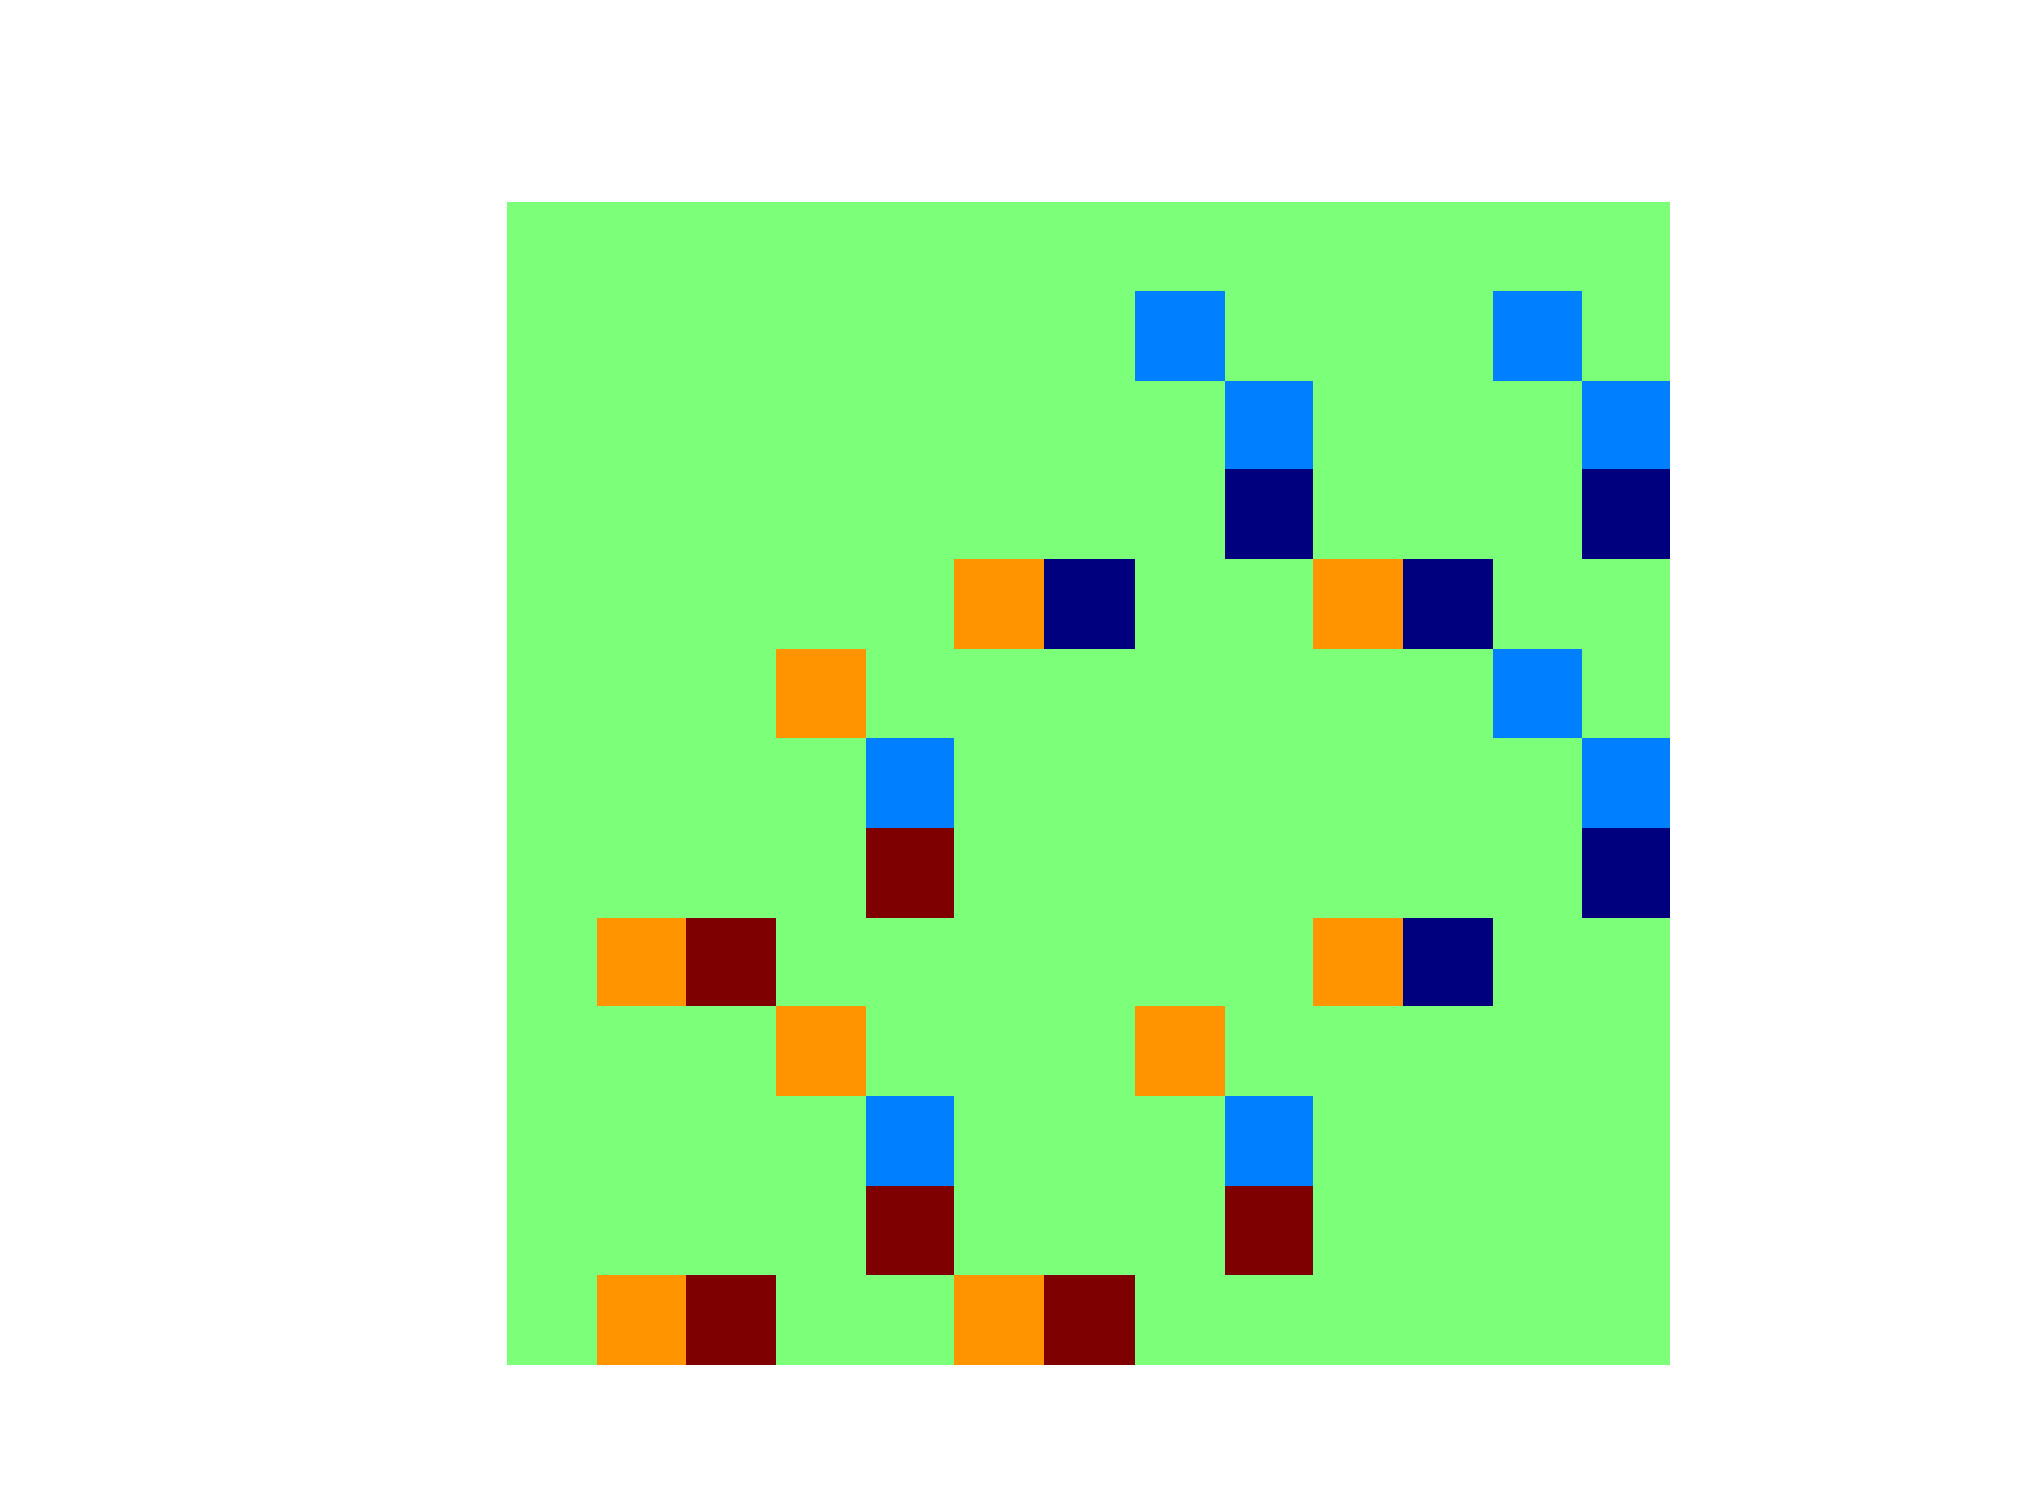
\includegraphics[width=5cm]{Kuhn3112_payoff.pdf}
  %%   \caption{\textbf{Left}: 2-simplex \textbf{Middle}: 7-simplex \textbf{Right}: 10-simplex}
  %% \end{figure}
\end{frame}

\begin{frame}
  \frametitle{Non-Linear Ledoit-Wolf: Why? How?}

  \begin{itemize}
  \item ($p/n$ large) or ($\Sigma$ eigenvalues close to one another)
    $\Rightarrow$ linear shrinkage OK.\\($p/n$ small) or ($\Sigma$
    eigenvalues dispersed) $\Rightarrow$ non-linear shrinkage better.
  \item Mar\v{c}enko-Pastur equation: relationship between $\B{S}$ and
    $\B{\Sigma}$ eigenvalues under large-dimensional asymptotics.
  \end{itemize}
\end{frame}

\begin{frame}
  \frametitle{Non-Linear Ledoit-Wolf: deeper into the "how?"}

  \begin{itemize}
  \item $H_n$ empirical d.f. of sample ($\B{S}_n$) eigenvalues $\B{\tau}_n$.\\
    $H_n(\B{\tau}) \equiv
    \frac{1}{p}\sum^p_{i=1}\mathbb{1}_{[\tau_i,+\infty[}(\tau)$
  \item $F_n$ e.d.f. of population ($\B{\Sigma}_n$) eigenvalues
    $\B{\lambda}_n$.\\$\B{Y}_n = \B{X}_n\B{\Sigma}^{1/2}_n$, $\B{X}_n
    \sim \mathcal{N}(\B{0},\text{Id})$
  \item $F_n$ (resp. $H_n$) converges almost surely to $F$ (resp. $H$).
  \item Stieltjes transform of a non-decreasing function $G$:
     $\forall z \in \mathbb{C}^+, m_G(z) \equiv
     \int^{+\infty}_{-\infty}\frac{1}{u - z}dG(u)$
   \item Mar\v{c}enko-Pastur equation: $\forall z \in \mathbb{C}^+,
     m_F(z) = \int^{+\infty}_{-\infty}\frac{1}{\tau[1-\frac{p}{n}-\frac{p}{n}zm_F(z)] - z}dH(\tau)$
  \end{itemize}
\end{frame}

\begin{frame}
  \frametitle{Non-Linear Ledoit-Wolf: Implementation\ldots}

  \begin{equation*}
    \begin{split}
      \textcolor{red}{Q_{n,p}}: & [0, \infty[^p \rightarrow [0,\infty[^p \\
              & \B{t} \equiv (t_1,\ldots,t_p)\trans
              \mapsto Q_{n,p}(\B{t}) \equiv
              (q^1_{n,p}(t),\ldots,q^p_{n,p}(t))\trans
    \end{split}
  \end{equation*}

  \vfill
  \hrule{}
  \vfill

  $\textcolor{blue}{\hat{\B{\tau}}_n} = \underset{\B{t} \in [0, \infty[^p}{\text{argmin}} 
      \frac{1}{p} \sum^p_{i=1}[\textcolor{red}{q^i_{n,p}(}\B{t}\textcolor{red}{)} - \lambda_{n,i}]^2$

  \vfill
  \hrule{}
  \vfill

  $\textcolor{PineGreen}{\overset{\smile}{m}^{\hat{\B{\tau}}_n}_{n,p}(}\lambda_i\textcolor{PineGreen}{)} \simeq \frac{n-p}{p\lambda_i} - \frac{n}{p}\frac{1}{\textcolor{blue}{\hat{\B{\tau}}_{n,i}}\lambda_i}$

  \vfill
  \hrule{}
  \vfill

  $\textcolor{purple}{\hat{d}_i^*} = \frac{\lambda_i}{|1 - \frac{p}{n} - \frac{p}{n}|^2\textcolor{PineGreen}{\overset{\smile}{m}^{\hat{\B{\tau}}_n}_{n,p}(}\lambda_i\textcolor{PineGreen}{)}}$; {\scriptsize Covariance:} $S_n^*\B{U}_n\textcolor{purple}{\hat{\B{D}}^*_n}\B{U}_n\trans${\scriptsize , with }$\B{S}_n=\B{U}_n\B{D}_n\B{U}_n\trans$
  
\end{frame}

\begin{frame}
  \frametitle{About the $Q_{n,p}$ function}

  \begin{equation*}
    \begin{split}
      Q_{n,p}: & [0, \infty[^p \rightarrow [0,\infty[^p \\
              & \B{t} \equiv (t_1,\ldots,t_p)\trans
              \mapsto Q_{n,p}(\B{t}) \equiv
              (\textcolor{red}{q^1_{n,p}(}t\textcolor{red}{)},\ldots,\textcolor{red}{q^p_{n,p}(}t\textcolor{red}{)})\trans
    \end{split}
  \end{equation*}

  \vfill
  \hrule{}
  \vfill

  $\forall i = 1, \ldots, p \quad \textcolor{red}{q^i_{n,p}(}t\textcolor{red}{)} \equiv
  p\int_{(i-1)/p}^{i/p}\textcolor{blue}{(F^{\B{t}}_{n,p})^{-1}(}u\textcolor{blue}{)}du$

  \vfill
  \hrule{}
  \vfill
  
  $\textcolor{blue}{(F^{\B{t}}_{n,p})^{-1}(}u\textcolor{blue}{)} \equiv \sup\{x \in \mathbb{R}: \textcolor{PineGreen}{F^{\B{t}}_{n,p}(}x\textcolor{PineGreen}{)} \leq u\}$

  \vfill
  \hrule{}
  \vfill
  
  $\textcolor{PineGreen}{F^{\B{t}}_{n,p}(}x\textcolor{PineGreen}{)} \equiv \max \left\{1 - \frac{n}{p}, \frac{1}{p}\sum^p_{i=1}\mathbb{1}_{\{t_i = 0\}}\right\}$ if $x = 0$, $\textcolor{PineGreen}{F^{\B{t}}_{n,p}(}x\textcolor{PineGreen}{)} \equiv \underset{\eta \rightarrow 0^+}{\lim}\frac{1}{\pi}\int^{+\infty}_{-\infty}\text{Im}\left[\textcolor{purple}{m^{\B{t}}_{n,p}(}\zeta + i\,\eta\textcolor{purple}{)}\right]d\zeta$ otherwise

  \vfill
  \hrule{}
  \vfill

  $m \equiv \textcolor{purple}{m^{\B{t}}_{n,p}(}z\textcolor{purple}{)}$ sol. in $\left\{m \in \mathbb{C}: -\frac{n-p}{nz} + \frac{p}{n}\right\}$ of $\textcolor{purple}{m} = \frac{1}{p}\sum^p_{i=1}\frac{1}{t_i(1 - \frac{p}{n} - \frac{p}{n}z\textcolor{purple}{m}) - z}$

\end{frame}

\end{document}
